%=============================Preamble=============================%
\documentclass[10pt,a4paper]{article}
\usepackage[T1]{fontenc}
\usepackage[utf8]{inputenc}
\usepackage[brazil]{babel}
%\usepackage[math]{anttor} % fonte um pouco mais estilizada
\everymath{\displaystyle}
\usepackage{import}
%\usepackage{parskip}
%=========================Packages==================================%
\usepackage{textcomp}
\usepackage{color,lscape, amsmath, hyperref, booktabs, latexsym, multicol, gensymb, lmodern, natbib, tikz, tkz-euclide, amssymb, enumitem, fancyhdr, lipsum, siunitx, setspace}
\usepackage{graphicx}

\newenvironment{Figure}
  {\par\medskip\noindent\minipage{\linewidth}}
  {\endminipage\par\medskip}

% configurações das questões, bem como: pontuação e estrutura.

\usepackage{tasks} % cria lista curta
\usepackage{exsheets} % cria questoes
\SetupExSheets[points]{name=ponto/s,number-format=\color{blue}} % define as configurações de pontuação das questões, e a cor da pontuação.

\DeclareInstance{exsheets-heading}{fancy-wp}{default}{
toc-reversed = true ,
indent-first = true ,
vscale = 2 ,
pre-code = \rule{\linewidth}{1pt} ,
post-code = \rule{\linewidth}{1pt} ,
title-format = \large\scshape\color{rgb:red,0.65;green,0.04;blue,0.07} ,
number-format = \large\bfseries\color{rgb:red,0.02;green,0.04;blue,0.48} ,
points-format = \itshape ,
points-pre-code = ( ,
points-post-code = ) ,
join =
{
number[r,B]title[l,B](.333em,0pt) ;
number[r,B]points[l,B](.333em,0pt)
} ,
attach = { main[hc,vc]number[hc,vc](0pt,0pt) }
}

%\SetupExSheets{headings=fancy-wp} % estilo diferente para o topo do enunciado com o nome " Exercício
%===========================Margins==============================%
\usepackage[top=8mm, bottom=20mm, left=8mm, right=8mm]{geometry}

%======================Cabeçalho e Rodapé========================%
\pagestyle{fancy}
\lfoot{\notaesquerda}
\cfoot{\thepage}
\rfoot{\notadireita}
%\lhead{HELLO}
%\chead{HELLO}
%\rhead{\textbf{The performance of new graduates}}
%\renewcommand{\headrulewidth}{0.4pt} %linha horizontal no topo da pagina
\renewcommand{\footrulewidth}{0.4pt} %linha horizontal no pé da pagina

\setlength\parindent{0pt}
\setlength\parskip{1.5ex}
\setlength\parsep{1.5\parskip}
%\thispagestyle{empty}%\bigskip %Rodapé na primeira pagina

\graphicspath{{figures/}} %informa a pasta em que as imagens estão
\usepackage{capt-of}%%To get the caption
\usepackage{amsmath}%
%=======================informações da atividade===============================%
\newcommand{\atv}{Lista de Exercícios 01 -- Noções de Conjuntos}
\newcommand{\preceptor}{Professor: Fernando Jorge}
\newcommand{\turma}{1º serie}
\newcommand{\bolsistas}{\atv \\ \preceptor}

%=====================informações de rodapé=================%
\newcommand{\notaesquerda}{Noções de Conjuntos
}
\newcommand{\notadireita}{Escola Estadual Professor Lima Castro}


\begin{document}

{\sf
  \begin{center}
     \textbf{\bolsistas
     }
  \end{center}
}\bigskip


\vspace{2mm}
\setlength{\marginparwidth}{5cm}
\small \noindent \textbf{Nome:}\hspace{0.3cm}\hrulefill \hrulefill
\hrulefill \hspace{0.1cm} 
\textbf{Número:}\hspace{0.1cm}\rule{1cm}{.1mm}


%\begin{center}
%\textsc{\Large Exercícios}    %Titulo do topo, antes de iniciar as questões
%\end{center}

	\begin{multicols}{2}

	  \setlength\columnseprule{0.6pt} % linha vertical entre as colunas
	  %\newpage %% ou \clearpage ou %% \pagebreak %% força uma quebra de pagina. caso os exercicios ocupem apenas metade de uma pagina.

    \begin{question}[type=exam]
      Represente na forma tabular cada um dos conjuntos \textbf{A}, \textbf{B} e \textbf{C} do diagrama abaixo.
        % \begingroup
        %   \centering
        %   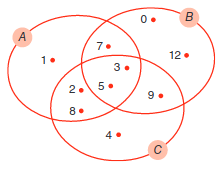
\includegraphics[scale=0.6]{figures/q1.png}
        % \endgroup
      \begin{Figure}
        \centering
        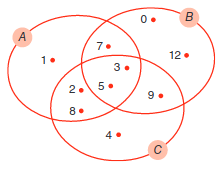
\includegraphics[scale=1]{figures/q1.png}
      \end{Figure}

    \end{question}
    
    \begin{question}[type=exam]
      Faça uma lista com todos os subconjuntos de $A = \big\{1,2,3\big\}$. 
    \end{question}

    \begin{question}[type=exam]
      Quantos subconjuntos possui o conjunto $E = \big\{a,e,i,o,u\big\}$?
    \end{question}

    \begin{question}[type=exam]
      Determine os números \textit{x} e \textit{y}, sabendo que $\big\{1,2,x\big\} = \big\{3,y,2\big\}$.
    \end{question}

    \begin{question}[type=exam]
      Dados os conjuntos $A = \big\{4,-3,-2,-1,0,1,2\big\}$, $B = \big\{0,1,2,3\big\}$, $C = \big\{-1,0,1,2,3,4\big\}$ e $D = \big\{3,4,5,6,7,8\big\}$, determine:
      \begin{tasks}(2)
        \task $A \cup B$
        \task $A \cap B$
        \task $A \cup D$
        \task $A \cap D$
        \task $A \cup B \cup D$
        \task $A \cap B \cap C$
        \task $A \cap B \cap C \cap D$
        \task $(A \cup D) \cap (B \cup C)$
        \task $(A \cap D) \cup (B \cup C)$
      \end{tasks}
    \end{question}

    \begin{question}[type=exam]
      Sabendo que $S \cap T = \big\{a,b,d\big\}$, $S = \big\{a,b,c,d\big\}$ e $S \cup T = \big\{a,b,c,d,e,f,g\big\}$, represente no diagrama abaixo os conjuntos \textit{S} e \textit{T}.
      \begin{Figure}
        \centering
        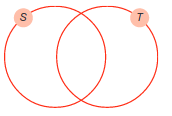
\includegraphics[scale=1]{figures/q6.png}
      \end{Figure}
    \end{question}

    \begin{question}[type=exam]
      Sabendo que $A \cap B = \big\{2,5\big\}$, $B = \big\{2,5,9\big\}$ e $A \cup B = \big\{2,3,5,8,9\big\}$, represente os conjuntos \textit{A} e \textit{B} por meio de um diagrama.
    \end{question}

    \begin{question}[type=exam]
      Determinar os conjuntos \textit{A} e \textit{B} tais que: $A - B = \big\{5,8,2\big\}$, $B - A = \big\{3,6\big\}$ e $A \cup B = \big\{1,2,3,5,6,7,8\big\}$.
    \end{question}

    \begin{question}[type=exam]
      Dados os conjuntos $E = \big\{3,8,6,4\big\}$, $F = \big\{1,2,3,8,6,4,9\big\}$ e $G = \big\{4,5,6,7,8\big\}$, determine:
      \begin{tasks}
        \task $F - E$
        \task $G - E$
        \task $(E \cup G) - F$
        \task $(F - G) \cup (G - F)$
      \end{tasks}
    \end{question}

    \begin{question}[type=exam]
      Sabendo que $A \cap B \cap C = \big\{0,6,8\big\}$, $A \cap B = \big\{0,6,8,1\big\}$, $A \cap C = \big\{0,6,8,12\big\}$, $B \cap C = \big\{0,6,8,2,3\big\}$, $B - A = \big\{2,3\big\}$,
      $C - B = \big\{12\big\}$ e $A - B = \big\{12,15\big\}$, represente os conjuntos \textit{A}, \textit{B}, \textit{C} em um diagrama como este:
      \begin{Figure}
        \centering
        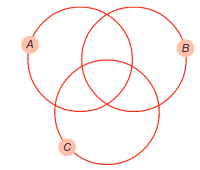
\includegraphics[scale=1]{figures/q10.png}
      \end{Figure}
    \end{question}

    \begin{question}[type=exam]
      O brasil é dividido em cinco regiões. 

      Considerando os conjuntos A = \{x|x é o estado da região Sul ou da região Nordeste do Brasil\}
      e B = \{y|y é o estado da região Nordeste ou da região Sudeste do Brasil\}:
      \begin{tasks}
        \task determine quais estados compõem o conjunto $A - B$. 
        \task determine quais estados compõem o conjunto $B - A$. 
      \end{tasks}

      \begin{Figure}
        \centering
        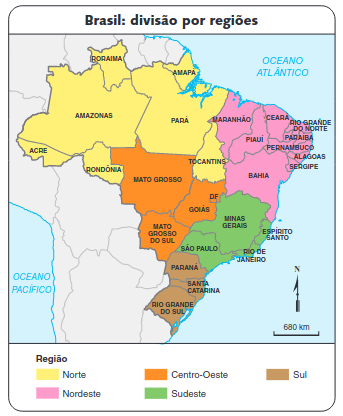
\includegraphics[scale=.7]{figures/q11.png}
      \end{Figure}
    \end{question}

    \begin{question}[type=exam]
      De uma pesquisa realizada pelo Ministério do Turismo com 2.200 gaúchos, pôde-se concluir que, precisamente: 

      \begin{itemize}
        \item 816 dos entrevistados já estiveram na região Nordeste do Brasil. 
        \item 602 dos entrevistados já estiveram na região Norte do Brasil. 
        \item 206 dos entrevistados já estiveram nas duas regiões. 
      \end{itemize}

      Quantas das pessoas entrevistadas nunca estiveram em nenhuma das duas regiões?
    \end{question}

    \begin{question}[type=exam]
      Um funcionário do departamento de Recursos Humanos de uma indústria automobilística, analisando o currículo de 47 candidatos
      a postos de trabalho, concluiu que apenas 3 deles nunca haviam trabalhado em montagem ou pintura, 32 já haviam trabalhado em 
      montagem e 17 já haviam trabalhado nos dois setores. Quantos desses candidatos haviam trabalhado apenas em pintura?
    \end{question}

    \begin{question}[type=exam]
      Uma fábrica de motocicletas realizou uma pesquisa de mercado com 400 jovens maiores de idade, concluindo
      que, precisamente:
      \begin{itemize}
        \item 283 dos entrevistados já haviam dirigido automóvel;
        \item 127 dos entrevistados já haviam dirigido motocicletas;
        \item 67 dos entrevistados não haviam dirigido nenhum dos dois tipos de veículo. 
      \end{itemize}

      Quantos dos jovens entrevistados já haviam dirigido os dois tipos de veículo?
    \end{question}

    \begin{question}[type=exam]
      Em uma empresa, 60\% dos funcionários têm mais de 20 anos de idade e 64\% têm menos de 40 anos de idade. 
      Qual é a porcentagem de funcionários dessa empresa com mais de 20 e menos de 40 anos de idade?
    \end{question}

    \begin{question}[type=exam]
      Cada um dos 51 professores de uma escola leciona em, pelo menos, um dos três prédios, A, B e C, que a escola possui. 
      A distribuição de aulas aos professores foi feita de modo que, precisamente:
      \begin{itemize}
        \item 32 professores lecionassem no prédio A;
        \item 30 professores lecionassem no prédio B;
        \item 29 professores lecionassem no prédio C;
        \item 17 professores lecionassem nos prédios A e B;
        \item 18 professores lecionassem nos prédios A e C;
        \item 13 professores lecionassem nos prédios B e C. 
      \end{itemize}

      Quantos professores dão aulas nos três prédios?
    \end{question}

    \begin{question}[type=exam]
      O número associado a cada ponto do eixo real é chamado de abscissa do ponto. Assim, os pontos A e B representados 
      no eixo real abaixo têm abscissas 3 e 5, respectivamente. 

      \begin{Figure}
        \centering
        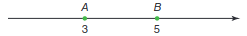
\includegraphics[scale=1]{figures/q17.png}
      \end{Figure}

      A distância \textit{d} entre A e B, também chamada de comprimento do segmento $\overline{AB}$, é a diferença entre as 
      abscissas de A e B, a maior menos a menor, isto é: $d = 5 - 3 = 2$. 

      Generalizando essa ideia para qualquer segmento de reta contido no eixo real:

      \begin{tasks}
        \task Calcule a distância entre os pontos E e F de abscissas 5 e 15, respectivamente.
        \task Calcule a distância entre os pontos C e D de abscissas $-4$ e 4, respectivamente. 
        \task Calcule a distância entre os pontos G e H de abscissas $\frac{3}{2}$ e $\frac{23}{4}$, respectivamente. 
        \task Determine a abscissa do ponto médio do segmento $\overline{IJ}$, em que \textit{I} e \textit{J} têm abscissas 5 e 9, respectivamente. 
        \task Determine a abscissa do ponto médio do segmento $\overline{KL}$, em que \textit{K} e \textit{L} têm abscissas $- \frac{1}{5}$ e $8$, respectivamente. 
      \end{tasks}

    \end{question}

    \begin{question}[type=exam]
      Dados os intervalos: $A = \big[4,12\big]$, $B = \big] 9,19\big[$, $C = \big]0,8\big]$ e $D = \big]- \infty,14\big]$, determine:

      \begin{tasks}(3)
        \task $A \cap B$
        \task $A \cup B$
        \task $B - D$
        \task $D - B$
        \task $A \cup B \cup C$
        \task $A \cap B \cap C$
      \end{tasks}
    \end{question}

    \begin{question}[type=exam]
      Sejam $A = \big]3,9\big]$ e $B = \big]5, +\infty\big[$. Sabendo que um número \textit{x} pertence a $A \cap B$, podemos concluir que \textit{x}
      não percente ao intervalo:

      \begin{tasks}(3)
        \task $\big[9,+\infty\big[$
        \task $\big]8,+\infty\big[$
        \task $\big[7,9\big]$
        \task $\big]-\infty,9\big[$
        \task $\big[10,15\big]$
      \end{tasks}
    \end{question}

    \begin{question}[type=exam]
      Quantos subconjuntos possui um conjunto com 8 elementos?
    \end{question}

    \begin{question}[type=exam]
      Um conjunto \textit{F} possui exatamente 128 subconjuntos. Qual é o número de elementos de \textit{F}?
    \end{question}

    \begin{question}[type=exam]
      Considerando os conjuntos \textit{A}, \textit{B} e \textit{C} de tal forma que $A \cup B = \big\{1,2\big\}$ e $A \cup C = \big\{1,2,3,4\big\}$,
      o conjunto $A \cup (B \cap C)$ será igual a: 

      \begin{tasks}(3)
        \task $A$
        \task $A \cup C$
        \task $\big\{3,4\big\}$
        \task $A \cup B$
        \task $\oslash$
      \end{tasks}
    \end{question}

    \begin{question}[type=exam]
      Se $A =\big]-2,3\big]$ e $B = \big[2,5\big]$, então os números inteiros que estão em $B - A $ são:
      \begin{tasks}(3)
        \task $-1$ e $0$
        \task 1 e 0 
        \task 4 e 5
        \task 3, 4 e 5
        \task 0, 1, 2 e 3
      \end{tasks}
    \end{question}

    \begin{question}[type=exam]
      Em uma escola, numa turma de 20 estudantes, 16 jogam futebol, 12 jogam voleibol e 2 não praticam esporte algum. 
      O número de alunos dessa turma que joga somente futebol é:
      \begin{tasks}(4)
        \task 4
        \task 6
        \task 10
        \task 12
      \end{tasks}
    \end{question}

    \begin{question}[type=exam]
      A Secretaria de Saúde do Estado da Paraíba, em estudos recentes, observou que o número de pessoas acometidas de 
      doenças como gripe e dengue tem assustado bastante a população paraibana. Em pesqusas realizadas com um universo
      de 700 pessoas, constatou-se que $10\%$ tiveram gripe e dengue, $30\%$ tiveram apenas gripe, e $50\%$ tiveram gripe 
      ou dengue. O número de pessoas que tiveram apenas dengue é:
      
      \begin{tasks}(5)
        \task 350 
        \task 280
        \task 210
        \task 140 
        \task 70
      \end{tasks}

    \end{question}

    \begin{question}[type=exam]
      Em um concurso público aplicado a 3.000 candidados, 2.300 obtiveram notas superiores ou iguais a 4,0, e 2.700 obtiveram 
      notas inferiores ou iguais a 6,0. Calcule o número de candidatos cujas notas foram:
      \begin{tasks}
        \task maiores ou iguais a 4,0 e menores ou iguais a 6,0;
        \task menores que 4,0.
      \end{tasks}
    \end{question}

    \begin{question}[type=exam]
      Numa pesquisa de mercado, verificou-se que 15 pessoas utilizam pelo menos um dos produtos A ou B. Sabendo que 10 dessas 
      pessoas não usam o produto B e que 2 dessas pessoas não usam o produto A, qual é o número de pessoas que utilizam os produtos
      A e B?
    \end{question}

    \begin{question}[type=exam]
      No início do ano letivo, o professor de Literatura sugeriu aos 1.210 alunos do ensino médio a leitura de três obras de Machado de Assis:
      \textit{Helena}, \textit{Dom Casmurro} e \textit{Quincas Borba}. No final do ano, o professor realizou um sondagem, com os mesmos 1.210 
      alunos, em que cada aluno respondeu "sim" ou "não" a cada uma das seguintes perguntas:

      \begin{enumerate}[label=\Roman*.]
        \item Você leu o romance \textit{Helena}, de Machado de Assis?
        \item Você leu o romance \textit{Dom Casmurro}, de Machado de Assis?
        \item Você leu o romance \textit{Quincas Borba}, de Machado de Assis?
      \end{enumerate}

      O professor tabulou os resultados da seguinte maneira:

      \begin{Figure}
        \centering
        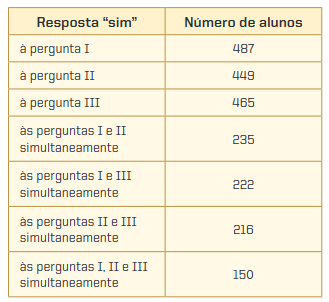
\includegraphics[scale=.8]{figures/q28.png}
      \end{Figure}
      De acordo com esses dados:

      \begin{tasks}
        \task quantos alunos leram apenas o romance \textit{Dom Casmurro}?
        \task quantos alunos responderam não às três perguntas?
      \end{tasks}

    \end{question}

    \begin{question}[type=exam]
      Uma pesquisa foi feita com um grupo de pessoas que frequentam, pelo menos, uma das três livrarias, A, B e C. Foram obtidos
      os seguintes dados:

      \begin{itemize}
        \item das 90 pessoas que frequentam a livraria A, 28 não frequentam as demais;
        \item das 84 pessoas que frequentam a livraria B, 26 não frequentam as demais;
        \item das 86 pessoas que frequentam a livraria C, 24 não frequentam as demais;
        \item 8 pessoas frequentam as três livrarias. 
      \end{itemize}

      \begin{tasks}
        \task Determine o número de pessoas que frequentam apenas uma das livrarias. 
        \task Determine o número de pessoas que frequentam, pelo menos, duas livrarias. 
        \task Determine o número total de pessoas ouvidas nessa pesquisa. 
      \end{tasks}

    \end{question}

    \begin{question}[type=exam]
      Um clube oferece a seus associados aulas de três modalidades de esporte: natação, tênis e futebol. Nenhum associado pôde se inscrever 
      simultaneamente em tênis e futebol, pois, por problemas administrativos, as aulas desses dois esportes serão dadas no mesmo horário. 
      Encerradas as inscrições, verificou-se que, dos 85 inscritos em natação, 50 só farão natação; o total de inscritos para as aulas de tênis 
      foi de 17 e, para futebol, 38; o número de inscritos só para as aulas de futebol excede em 10 o número de inscritos só para as de tênis. 
      Quantos associados se inscreveram simultaneamente para aulas de futebol e natação?

    \end{question}

		\clearpage
	\end{multicols}
        
  %\import{questions/}{q7} % exemplo para mostrar que pode colocar questões fora das colunas e mesclar os estilos. Recomendado adicionar questões que incluem imagens, ao final e fora das colunas.
          





\end{document}
